\chapter{Introduction}
\label{chap:Introduction}

\section{Data-intensive applications}

Data-intensive applications fall into 2 computing styles
\begin{itemize}
  \item Internet-service (cloud-computing)
  \item High-performance computing (HPC)
\end{itemize}
In both cases, the underlying file system is a key component for scalable
application performance (Chap.\ref{chap:file_system}). At a higher-level, data is organized into a logical data warehouse called database.
There are different types of databases - Sect.\ref{sec:database_categories}, and each type has different implementations from different vendors.

\section{Different data models}

The different data models are given in Fig.\ref{fig:data_models}
\begin{enumerate}
  \item Relational data model
  
  \item Hierachical data model
  
  \item Graph data model
\end{enumerate}

\begin{figure}[hbt]
  \centerline{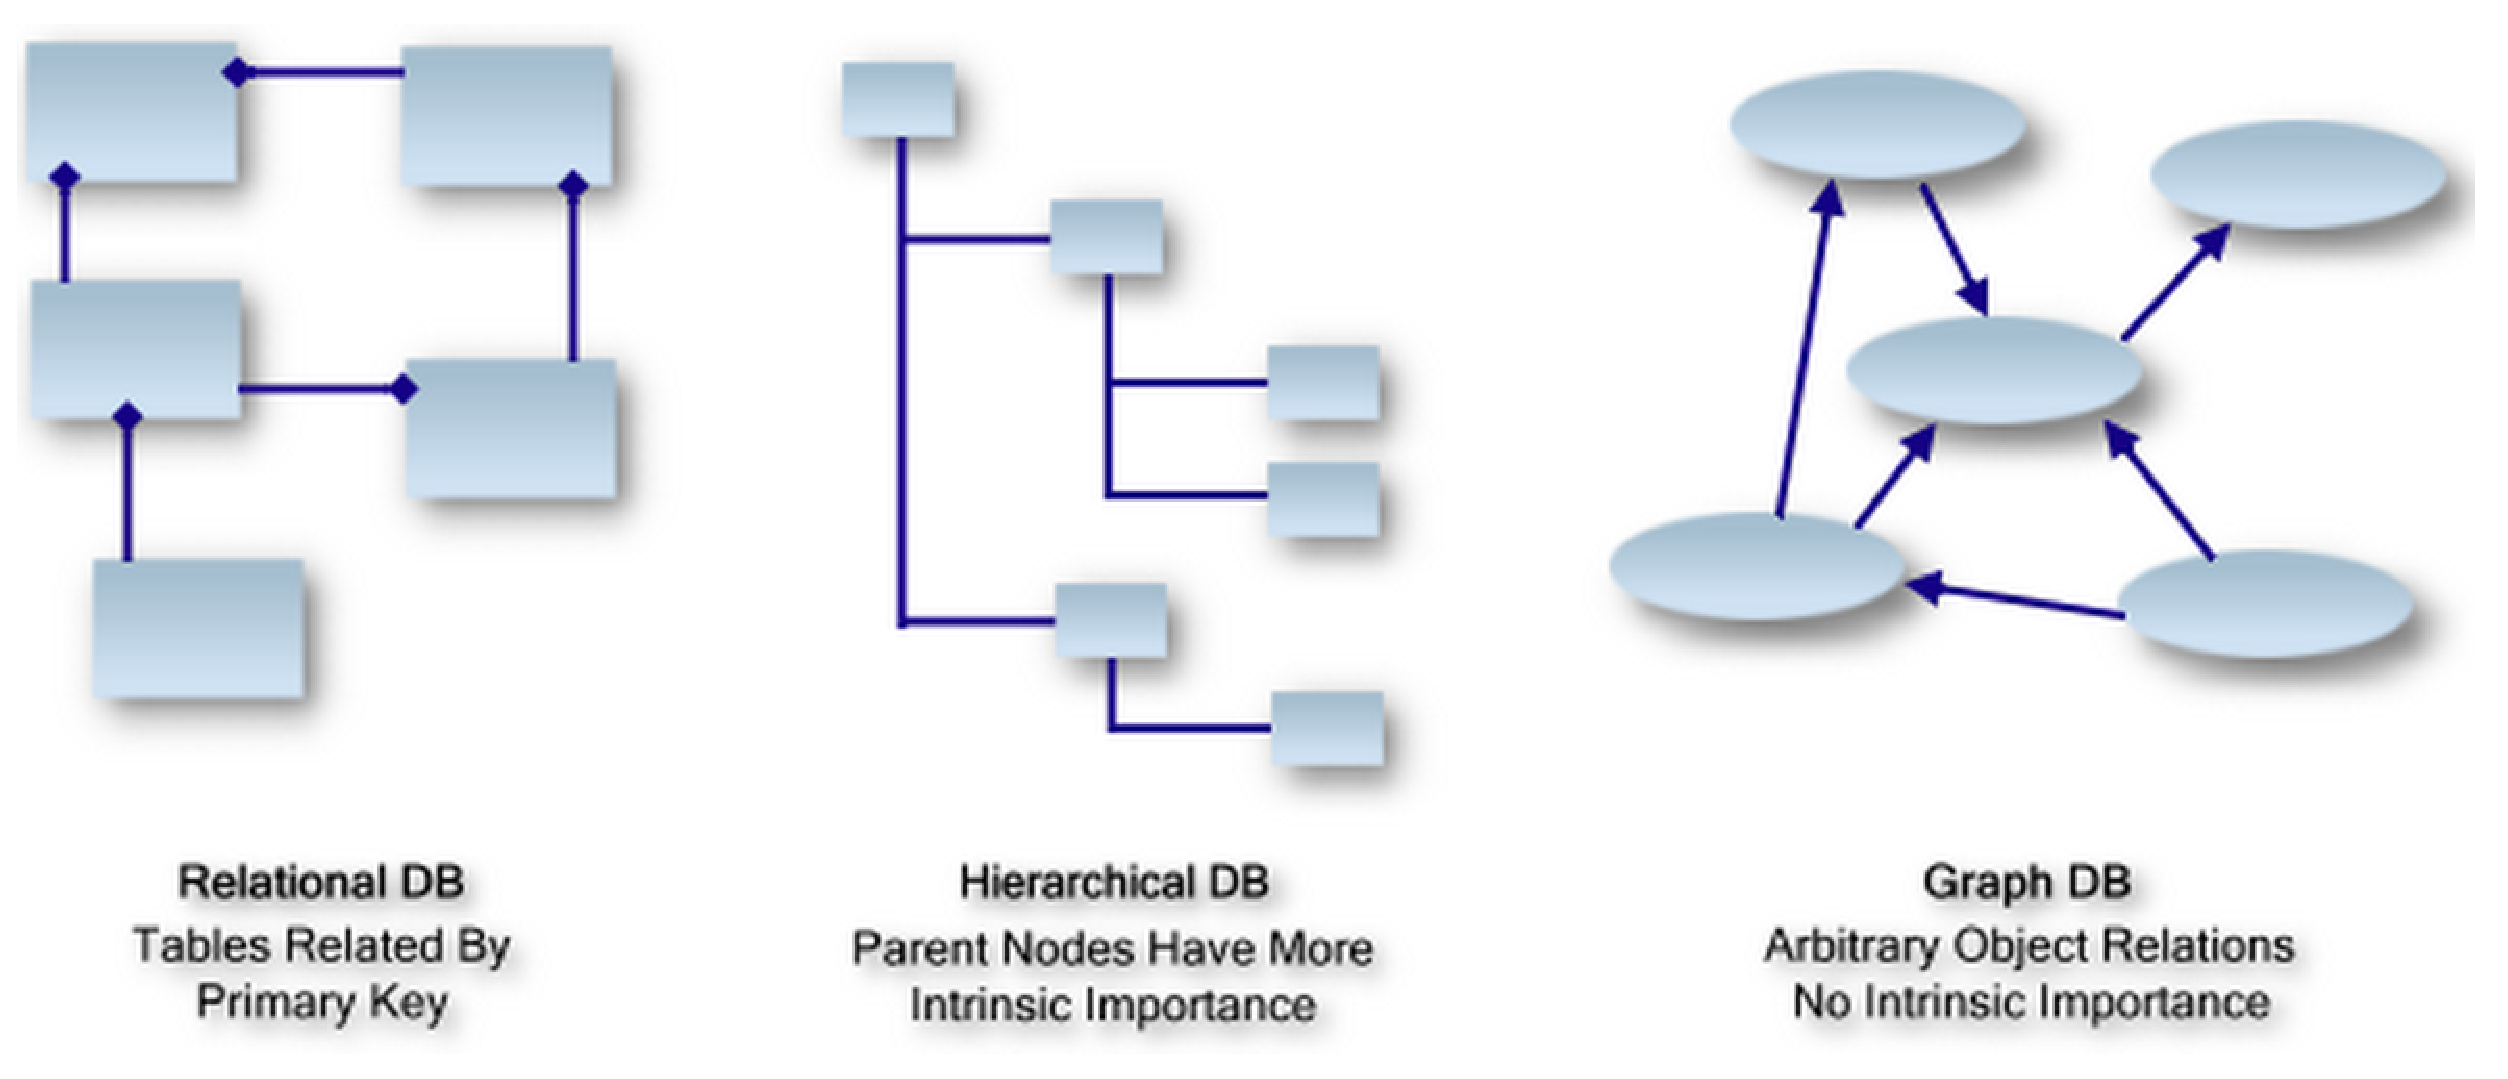
\includegraphics[height=7cm,
    angle=0]{./images/data_models.eps}}
  \caption{(A) Relational DB (tables related by primary keys), (B) Hierachical DB (parent nodes), (C) Graph DB (arbitrary object relations)}
  \label{fig:data_models} 
\end{figure}


\section{RDBMS vs. NoSQL vs. Graph vs. Cloud databases}
\label{sec:database_categories}

Relational Database Management System (RDBMS) organizes data into tables (each
row is a record, and each column represents a field; with metadata containing
the constraints expressing the relation between these tables) and uses SQL
language to query data (Chap.\ref{chap:SQL_lang}).
As the result, the structure of the database is described using well-structured
schemas. Read Sect.\ref{sec:RDBMS}

NoSQL-like databases do not use SQL-language, and suppor unstructured data, i.e.
the number of columns can be different at diffferent rows in one
table/docucment/object. In addition to table, other concept can be used, e.g.
documents, objects. A NoSQL database can be local, e.g. BerkeleyDB or
distributed, e.g. HBase, MongoDB. It can be classified into
\begin{itemize}
  \item object-oriented: Sect.\ref{sec:NoSQL_object-oriented}
  \item document-oriented: Sect.\ref{sec:NoSQL_document-oriented}
\end{itemize}

A {\bf graph database} is a database that uses graph structures for semantic
queries with nodes, edges and properties to represent and store data.
Every element contains a direct pointer to its adjacent elements and no index
lookups are necessary. Read Sect.\ref{sec:Graph_database}.


A cloud database is a database that typically runs on a cloud computing platform. 
This is not a new form of database, i.e. the database can be any of the above type. 
Read Sect.\ref{sec:Cloud_database}.

 


\section{RDBMS}
\label{sec:RDBMS}

RDBMS was first introduced in 1969 by Edgar F. Codd.
\begin{enumerate}
  \item it is a group of tables
  \item each table contains rows, columns and primary key
  \item relationship between tables are maintained using foreign key
  \item query language: SQL
\end{enumerate}

SQL was first introduced for Edgar F. Codd's relational model
(Chap.\ref{chap:SQL_lang}).

To guarantee database integrity when changing the data, {\bf database
transactions} are defined. Properties are ACID
\begin{itemize}
  \item Atomicity: the operations on database for a single transaction either
  all occur or nothing
  
  \item Consistency: ensure the integrity constraints during database operations
  \item Isolation: one operation is invisible to other concurrent operation
  \item Durability: ensure the transaction survive permanently
\end{itemize}


To optimize database structure, {\bf database normalization} is required
\begin{enumerate}
  \item organize tables and fields to minimize redundancy and dependency
  
  Devidie large tables into small tables with relations: 1NF, 2NF, 3NF, BCNF
  (Boyce-Codd Normal Form)
  
  \item a RDBMS is described as normalized if it is in 3NF (third normal form)
\end{enumerate}
Without normalization, it becomes difficult to handle and update database,
without facing data loss.

1NF = no two rows of data contains repeating group of information. So, each
table should have a unique value for each row, known as {\bf primary key}. The
primary key values are usually organized into a single column.

2NF = there is no partial dependency of any column on primary key. When a table
have more two or more columns as primary key (i.e. concatenated primary key),
then the value in each column that is not part of the primary key must depend
upon the entire concatenated key, not just part of it.

3NF = every non-prime attribute of the table must depend on the primary key. The
{\it transitive functional dependency} should be removed from the table.
Example:
\begin{verbatim}
Student_id   Student_name  DoB  Street city State Zip
\end{verbatim}
Here, street, city and state depend on zip. The dependency between Zip column
and other fields is called transitive dependency. Thus, a new table must be
created.

BCNF = a higher version of 3NF, in which a 3NF table that doesn't have multiple
overlapping candidate key is said to be in BCNF.

\begin{figure}[hbt]
  \centerline{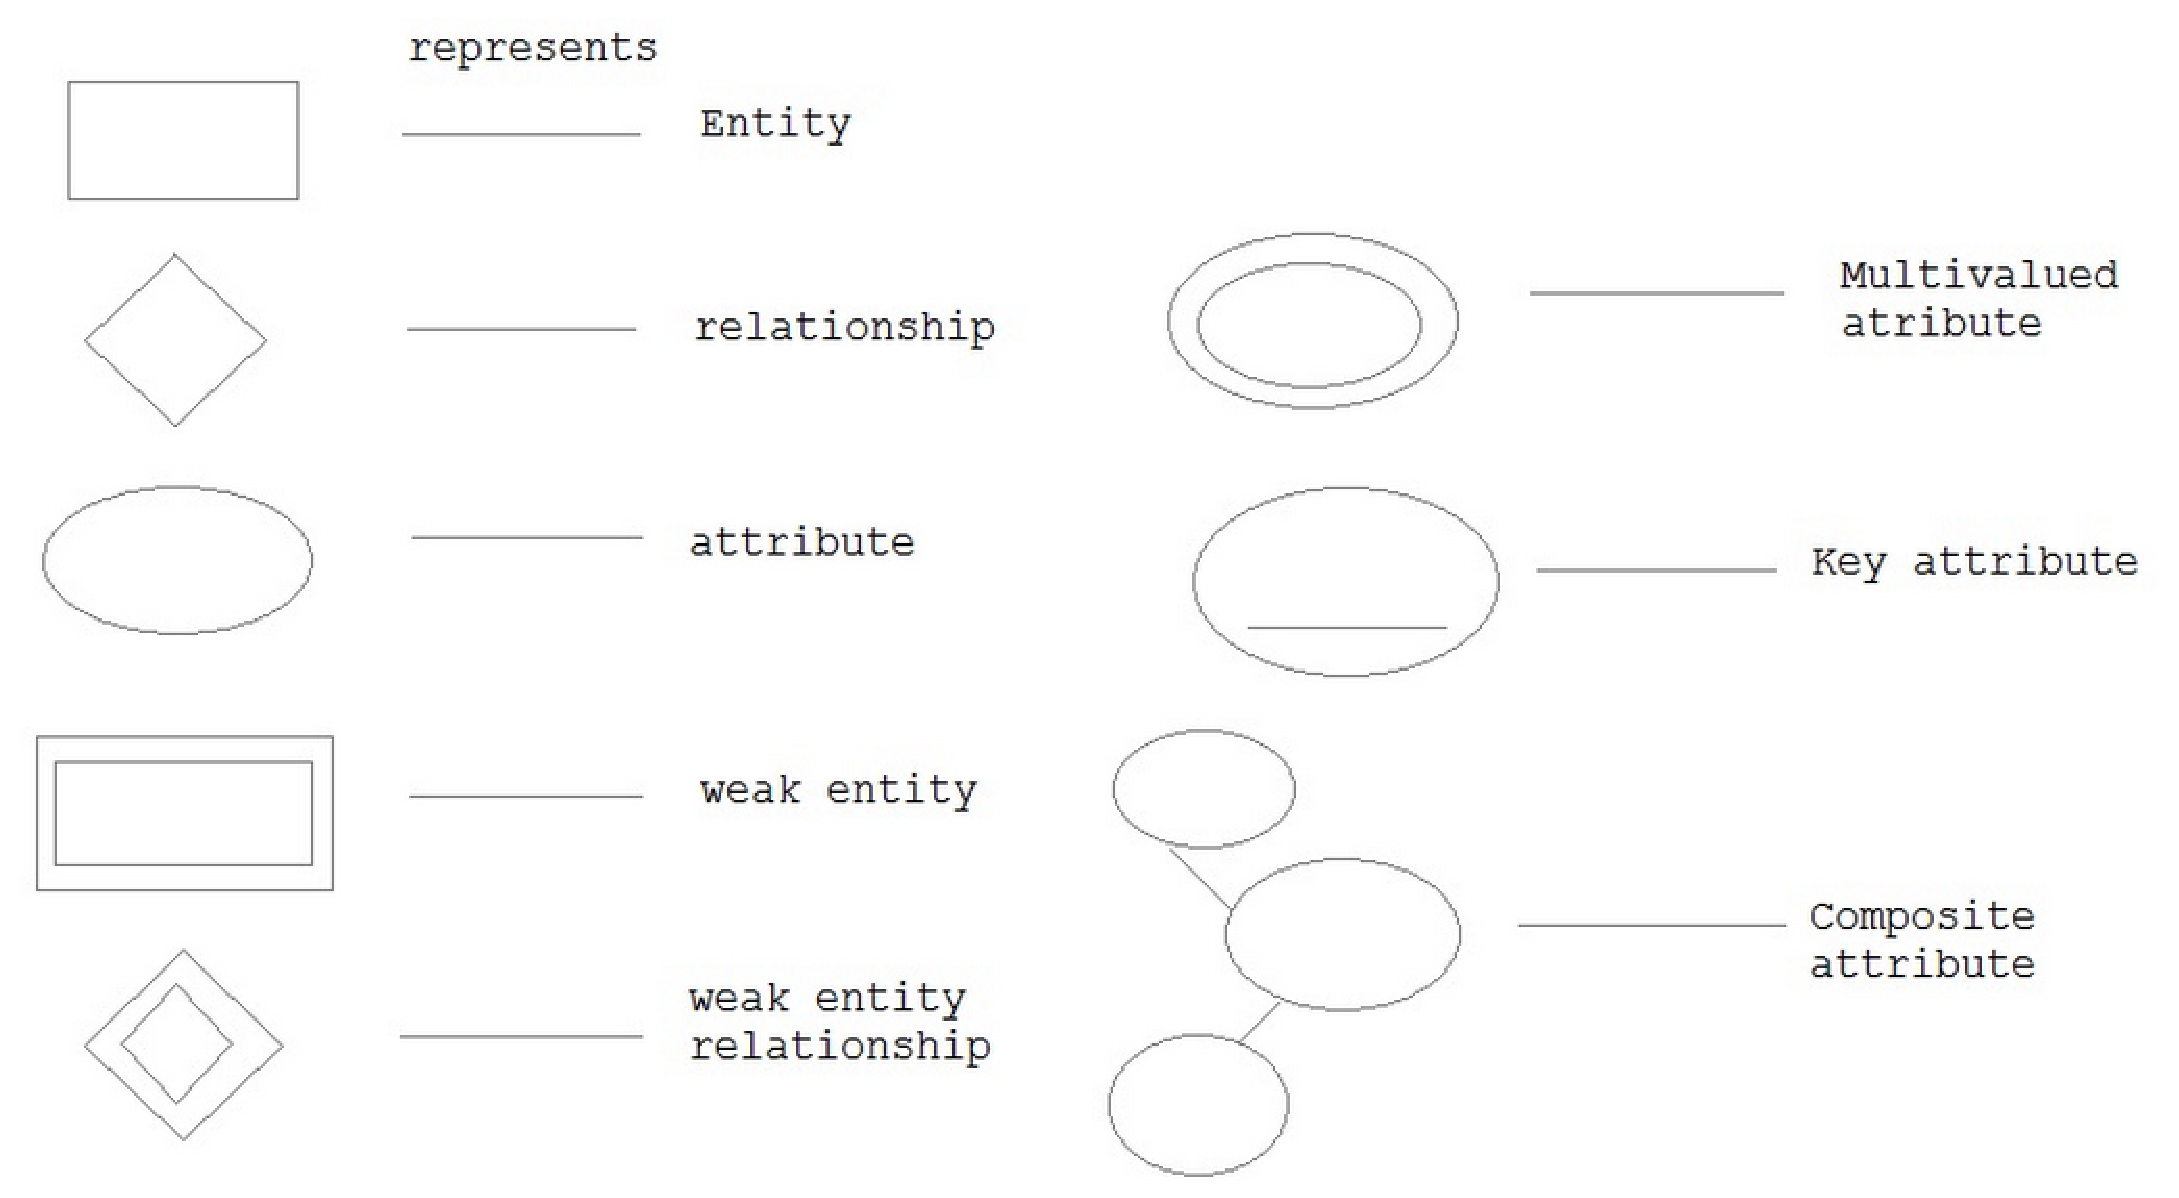
\includegraphics[height=6cm,
    angle=0]{./images/table-relationship.eps}}
\caption{Table relationship used in E-R diagram}
\label{fig:table-relationship}
\end{figure}

The relationship (dependency) between tables is represented using E-r diagram,
Fig.\ref{fig:table-relationship}.
\url{http://www.studytonight.com/dbms/er-diagram.php}

%\subsection{Softwares}

These software use SQL language to query/change data
\begin{enumerate}
  \item MySQL
  \item Microsoft SQL Server
  \item Oracle
  \item Infomix
  \item Sybase
  \item MS Access
  \item MariaDB
  \item PostgreSQL
\end{enumerate}

\subsection{Oracle}
The first commercial SQL based RDBMS is Oracle in 1977 when Lary Ellison first
saw a paper from IBM Journal of Research and Development that describes a
prototype for a RDBMS. He and coworkers Bob Miner and Ed Oates at Ampex formed
the Oracle company.
\begin{itemize}
  \item Oracle 1 (1978) written in assembly, never released
  \item Oracle 2 (1979)
  \item Oracle 3 (1983) written in C, first to run on mainframes, minicomputer
  and PCs
  \item Oracle 5 (1985) first to support client-server environment
  \item Oracle 6 (1988) allow multi-users to work on a single table, hot-backup,
  PL/SQL allow users to process data while it remains on databse
  
  \item Oracle 7 (1992) made major changes to structure and functions
  
  \item Oracle 7.3 (1996) support any type of data (text, video, map, sound,
  images)
  
  \item Oracle 9i (2001) improve performance, scalability and availability by
  allowing customers to use low-cost servers with Oracle Real Application
  Clusters
  
  \item Oracle 10g (2003) the first grid-computing product for enterprise, i.e.
  process the load based on demand
  
  \item Oracle 11g (2007) fast, reliable, secure and easys to manage all types
  of database workloads (enterprise applications, data warehouse, bid data
  analysis)
\end{itemize}
\url{http://www.slideshare.net/BcomBT/latest-trends-in-database-management}

\subsection{Microsoft SQL Server}

Microsoft SQL server
\begin{itemize}
  \item SQL Server 1.0 (1989): 16-bit
  \item SQL Server 1.1 (1991): 16-bit
  \item SQL Server 4.21 (1993): 
  \item SQL Server  6.0 (1995): 
  \item SQL Server 6.5 (1996)
  \item SQL Server 7.0 (1998)
  \item SQL Server 2000 (2000)
  \item SQL Server 2000 (2003): 64-bit
  \item SQL Server 2005 (2005): 
  \item SQL Server 2008 (2008)
  \item SQL Azure DB (2010): cloud-database
  \item SQL Server 2012 (2012): provide Mission Critical Confidence (greater
  uptime, fast performance and enhanced security features for mission critical
  workloads), Breakthrough Insight (managed self-service data exploration,
  stunning interactive data visualization capabilities)	
  \begin{itemize}
    \item data any types (structured or unstructured)
    \item any size (GB to PB)
    \item connecting with external data source (US Census Bureau, U.N.)
  \end{itemize}
\end{itemize}

\subsection{MySQL}

MySQL (most popular open-source RDBMS)
\begin{itemize}
  \item MySQL 1.0 (1994): originally developed by Michael Widenius and David
  Axmark
  \item MySQL 3.19 (1996)
  \item MySQL 3.21 (1997)
  \item MySQL 3.22 (1998)
  \item MySQL 3.23 (2000)
  \item MySQL 4.0 (2002)
  \item MySQL 4.01 (2003)
  \item MySQL 4.1 (2004)
  \item MySQL 5.0 (2005)
  \item 2008: acquired by Sun MicroSystems
  \item MySQL 5.1 (2008)
  \item 27-Jan-2010: Oracle acquired Sun MicroSystems
  \item MySQL 5.5 (2010)
  \item MySQL 5.6 (2011): enable next generation web-based and embedded
  applications and services
\end{itemize}

\subsection{MariaDB}

MariaDB (open source) created by some of the original authors of MySQL, lead by
Michael Widenius
\begin{itemize}
  \item MariaDB 5.1 (2009)
  \item \ldots
  \item MariaDB 10.0.0 (2012): 
  \begin{itemize}
    \item more storage engine than MySQL
    \item speed better than MySQL
    \item new features: GIS functionality, etc.
    \item truly open source
  \end{itemize}
\end{itemize}

\subsection{PostgreSQL}

PostgreSQL (most advanced open-source RDBMS): ACID-compliant
\begin{itemize}
  \item PostgreSQL 1.0 (1996)
  \item PostgreSQL 6.0 (1997)
  \item PostgreSQL 7.0 (2000)
  \item PostgreSQL 8.0 (2005)
  \item PostgreSQL 9.0 (2010)
  \begin{itemize}
    \item object-relational database system
    \item nested transactions
    \item international character sets
    \item spatial database for GIS
\end{itemize}
\end{itemize}

\subsection{Amazon Aurora}
\label{sec:Aurora}

\subsection{NuoDB}
\label{sec:NuoDB}


\section{Distributed Databases}

A distributed database is a database in which a storage devices are not all
attached to a common processing unit such as the CPU, i.e. 
collections of data (e.g. in a database) are distributed across multiple
physical locations (e.g. on the Internet, on the corporate intranets, etc.).

\section{NewSQL}
\label{sec:NewSQL_database}

This is a new idea proposed in 2011. As NoSQL solutions cannot give up strong
transactional and consistency requirement like SQL, to deal with large financial
and order processing systems the only options previously available for these
organizations were to either (1) purchase a more powerful single-node machine or
(2) develop custom middleware that distributes queries over traditional DBMS
nodes. Both are prohibitively expensive and only a few big companies can affort.

NewSQL combines the power of NoSQL and maintains ACID property of SQL.
There are two types
\begin{enumerate}
  \item  completely new database platforms (redesign from scratch): each node
  keeps a subset of the data, i.e. share nothing nodes. 
  
  Examples: 
   Google Spanner, Clustrix, VoltDB, MemSQL, Pivotal's SQLFire and GemFire XD,
  SAP HANA, FoundationDB, NuoDB, TransLattice, ActorDB, and Trafodion.
  
  \item optimize storage engine for SQL: 
  
  Example:  TokuDB and InfiniDB.
\end{enumerate}

\url{http://en.wikipedia.org/wiki/NewSQL}

\subsection{TokuDB}
\label{sec:TokuDB}

\subsection{InfiniDB}
\label{sec:InfiniDB}

\subsection{VoltDB}

\subsection{MemSQL}

\subsection{ActorDB}

\subsection{Google Spanner}

\subsection{Clustrix}

\subsection{Pivotal's SQLFire + GemFire XD}	

\subsection{SAP HANA}

\subsection{FoundationDB}

\subsection{NuoDB}

\subsection{TransLattice}

\subsection{Trafodion}


\section{Cloud database (CDBMS)}
\label{sec:Cloud_database}

A cloud database is the one that runs on a cloud computing platform (large
number of computers interconnected through a real-time communication network,
e.g. Internet) (Sect.\ref{chap:cloud_computing}). 
A cloud database can be either a SQL-based or no-SQL-based data model. In other
words, a traditional database or NoSQL can be extended to support cloud. The
major drawback is {\bf security} and {\bf privacy issues}. 


There are three methods to run a database on the cloud:
\begin{itemize}
  \item using virtual machine image: user purchase a machine instance, for a
  limited time, and run the database with optimized-installation on these
  machine. user can also have the option to upload their own machine image
  with a database installed onit.
  
  In any way, the user still need to control and manage their database.
  
  \item Database as-a-Service (DBaas): the user do not need to install or
  maintain the database. Instead, the database service provider takes
  responsibility for installing and maintaining the database, and the user pay
  according to their usage.
  
  \item The database, even though hosted on the cloud, but is not offered as a
  service. The user can ask the cloud provider to manage it on the user's
  behalf. SQL databases are difficult to scale, meaning they are not natively
  suited to a cloud environment, although there are attempts to address this
  challenge for SQL-based database service. NoSQL databases are more
  suitedfor the cloud as it can scale up/down easily.
  
  Example: service by Rackspace (manage hosting for MySQL or NoSQL on dedicated
  and cloud architectures), service by Object Rocket (manage hosting for
  MongoDB)
\end{itemize}

The following companies provide services belong to one of the three categories
above
\begin{enumerate}
  \item MongoLab
  \item Microsoft SQL Azure DB
  
  \item Rackspace Cloud Database
  \item Amazon RDS: 3 database services (SimpleDB, Amazon RDS,
  DynamoDB)
  
  \item Google Cloud SQL
  \item Oracle Cloud
  \end{enumerate}

\subsection{Rackspace Cloud}

It use MySQL database, built on OpenStack (open source software cloud computing
software platform - Sect.\ref{chap:OpenStack}).

\subsection{Amazon Cloud}

Amazon RDS (Relational Database Service) give us accesses to the familiar MySQL,
Oracle or Microsoft SQL Server database engine. This can be done via different
DB Instance class.


Each customer has an instance with pre-configured parameters, automated backup

\subsection{Google Cloud}

Google Cloud allows customers to create, configure and use a RDBMS that live in
the Cloud.
\begin{itemize}
  \item easy-to-use:
  \item exceptional security
\end{itemize}


\subsection{MongoLab}



\subsection{Microsoft SQL Azure DB}

SQL Azure DB (2010)



\section{NoSQL (document-oriented)}
\label{sec:NoSQL}
\label{sec:NoSQL_document-oriented}

NoSQL is useful when working with huge quantitaty of data (e.g. big data) when
the data nature does not require a relational model. NoSQL provides mechanism to
store and retrieve data that use looser consistency models than traditional
RDBMS. Example: Hadoop, MongoDB, CouchDB, Oracle NoSQL Database, OrientDB,
Apache Cassandra.

So, NoSQL doesn't focus on the relationship between elements; but the capability
to store and retreieve great quantitatives of data. 
\begin{itemize}
  \item elastic scaling: low-cost commodity hardware, scaling easy
  \item big data:
  \item economics: use clusters of cheap commodity servers to manage the
  exploding data and transaction volumes
  \item flexible data model: more relaxed or even nonexistent data model
  restrictions
\end{itemize}


Current challenges
\begin{itemize}
  \item relatively new compared to RDBMS: many key features have yet be
  implemented
  \item support: most NoSQL projects are open-source
  \item few features to support analytics and business intelligence: even simple
  queries requires significant programming expertises
  \item administration: current NoSQl requires strong skills to install and to
  maintain
  \item not many experts: almost every NoSQL developer is in learning mode
\end{itemize}

Key datatypes in NoSQL
\begin{verbatim}
Key-value pair
Wide column
Graph
Document
Object
XML
\end{verbatim}

Document-oriented No-SQL databases can use either of the following format as
the native format:
\begin{itemize}
  \item XML: BaseX (Sect.\ref{sec:BaseX}), eXistDB (Sect.\ref{sec:eXistDB}),
  MarkLogic (Sect.\ref{sec:MarkLogic}), Sedna (Sect.\ref{sec:Sedna})
  
 These databases use XML as an interface to specify documents as tree structured
 data that may contain unstructured text, but on disk the data is stored as
 {\bf "optimized binary files."} This makes query and retrieval faster.
MarkLogic also allows XML and JSON to co-exist in one binary format.  
  
  \item JSON: 
\end{itemize}

NOTE: Some RDBMS databases also support handle XML type query, e.g.
\begin{verbatim}
SELECT
   id, vol, xmlquery('$j/name', passing journal AS "j") AS name
FROM
   journals
WHERE 
   xmlexists('$j[licence="CreativeCommons"]', passing journal AS "j")
\end{verbatim}
though using the native format of XML or JSON is faster.

\subsection{MongoDB}
\label{sec:MongoDB}

MongoDB (open-source, currently the most popular NoSQL) developed by 10gen in
Oct, 2007.
\begin{itemize}
  \item store structured data as JSON-like documents with dynamic schemas
  (format: BSON): make the integration of data in certain types of application
  easier and faster. It doesn't use table, but collection concept (wrapped by
  \verb!{  }!)
  
  As you can see, it is document-oriented storage
  \begin{verbatim}
{
"_id" : ObjectID("...."),
"Last name": "Dumont",
"First name": "Jean",
"DoB": "01-11-2010"
},

{
...
}
  \end{verbatim}
  
  \item SQL support? No
  
  query language: a rich, ad-hoc query language of its own
  (don't use SQL language)
  
  \item used by: MTV Networks, FourSquares, UIDA
\end{itemize}

When to use
\begin{itemize}
  \item general-purpose design: content management system, mobile applications,
  gaming, e-commerce, analytics, archiving, and logging
  
  \item don't require ACID transactions; yet provide some basic transactional
  capabilities with atomic operations.
  
  \item write in MongDB can be 'D'urable.
\end{itemize}

When not to use
\begin{itemize}
  \item systems that require SQL, joins, and multi-oriented transactions
\end{itemize}

\subsection{CouchDB}
\label{sec:CouchDB}

Apache CouchDB (open source) first released in 2005, and become Apache project
in 2008
\begin{itemize}
  \item use JSON-like format: store data as a collection of independent
  documents
  
  \item Javascript as the query language: a database system that completely
  embrace the web
  
  \item ACID semantics
  
  \item Security and Validations
  
  \item Distributed Updates and Replications
\end{itemize}


\subsection{Riak}
\label{sec:Riak}



\subsection{Oracle NoSQL database}

Oracle NoSQL 
\begin{itemize}
  \item a distributed key-value database
  
 data is stored as key-value pairs
 
 \item No Single Point of Failure design: ensure the system continues to run and
 data remain available after any failure
\end{itemize}

\subsection{OrientDB}

OrientDB (open source) written in Java
\begin{itemize}
  \item use JSON-like format:
  
  \item GraphDB: native management of graphs 
   
  A document-based database system, but the relationships are managed as
  in graph databases with direct connections between records
  
  \item amazing fast: store 150,000 records per second on common hardware
  
  \item support advanced features: ACID transactions, fast indexes, native and
  SQL queries
  
  \item support SQL? Yes with extensions to handle relationship without SQL join
  
  \item Web-ready: natively support HTTP, RESTful protocol, JSON without 3rd
  party libraries and documents
  
  \item run everywhere: pure 100\% Java
\end{itemize}

\subsection{Apache Cassandra}

Apache Cassandra (open source), a top-level project of Apache
\begin{itemize}
  \item initially developed by Facebook to power their Inbox Search feature
  until late 2010
  
  released as an open source project on Google code (Jul-2008). became an Apache
  Incubator project in Mar-2009; and got to top-level project in Feb-2010.
  
  \item distributed database management system
  \item fault-tolerance: data is replicated to multiple nodes
  \item performant: outperform popular NoSQL alternatives
  \item decentralized: no single point of failures $\rightarrow$ durable
  (suitable for applications that can't afford loss of data)
  
  Every node in the cluster are identical $\rightarrow$ not suitable for very
  large database
\end{itemize}

\subsection{Amazon DynamoDB}
\label{sec:DynamoDB}


Amazon DynamoDB is a no-SQL database engine developed by Amazon to use on their
EC2 cloud compute platform. However, there is a version to be downloaded and use
on local system to test DynamoDB-backed applications locally.


DynamoDB exposes a similar data model and derives its name from Dynamo, but has
a different underlying implementation. Dynamo had a multi-master design
requiring the client to resolve version conflicts and DynamoDB use synchronous
replication across multiple datacenters for high durability and
availability.

\subsection{ArangoDB}
\label{sec:ArangoDB}


\subsection{BaseX}
\label{sec:BaseX}

\subsection{eXistDB}
\label{sec:eXistDB}

\subsection{MarkLogic}
\label{sec:MarkLogic}

\subsection{Sedna}
\label{sec:Sedna}

Sedna is a free native XML database which provides a full range of core database
services - persistent storage, ACID transactions, security, indices, hot backup.
Flexible XML processing facilities include W3C XQuery implementation, tight
integration of XQuery with full-text search facilities and a node-level update
language.

Sedna is designed with the goal of providing a balance in performance between
XML queries and updates execution.
\url{http://www.sedna.org/}

\section{NoSQL (object-oriented)}
\label{sec:NoSQL_object-oriented}

\subsection{NeoDatis}

NeoDatis ODB which is an object-oriented database (not a document-oriented like
CouchDB or MongoDB). It has a very low memory footprint and supports database file encrytption.

\url{http://stackoverflow.com/questions/2516752/anyone-using-nosql-databases-for-medical-record-storage}

\section{Graph Database}
\label{sec:Graph_database}

The graph database is the data storage model used by semantic Web
(Chap.\ref{chap:GraphData_LargeScale}).


\section{Search engine}
\label{sec:search_engines}

Popular search engines are given in
\url{http://db-engines.com/en/ranking/search+engine}

\begin{enumerate}
  \item Solr (Sect.\ref{sec:Solr})
  \item ElasticSearch
  \item Splunk
  \item Sphinx
  \item Endeca
  \item MarkLogic
  \item Google Search
\end{enumerate}
Chap.\ref{chap:Desktop_SearchEngine} and Chap.\ref{chap:Web_SearchEngines}

\section{NoSQL (multi-model)}

A NoSQL multi-model database provide both document-oriented, object-oriented,
graph-oriented, key-value, Schema-less
\begin{itemize}
  \item OrientDB
  \item ArangoDB

\url{http://vschart.com/compare/arangodb/vs/orientdb}


\end{itemize}



\section{MapReduce}
\label{sec:MapReduce}

MapReduce is a distributed programming model introduced by Google which
typically requires a distributed filesystem, and an associated database system 
\begin{enumerate}
  \item Google MapReduce: use Google Bigtable database
  (Chap.\ref{chap:google_bigtable}) on Google Distributed Filesystem (GDFS)
  \item Apache Hadoop (Sect.\ref{chap:Hadoop}): use Hadoop file system (HDFS)
  with HBase database
  
  HBase features data compression, in-memory operation and Bloom filter.
  However, it is not as performant as HDFS in a MapReduce context, and can be 4
  to 5 times slower.

  \item Couchdb (Sect.\ref{sec:CouchDB})
  \item Infinispan
  \item MongoDB (Sect.\ref{sec:MongoDB})
  \item Riak
\end{enumerate}

Unlike MPI, MapReduce is designed for cloud-based distributed system, that can
deals with fault tolerance, and the large datasets are splitted into smaller,
more manageable size, which are then processed by multiple {\bf map} instances.
The results produced by individual {\bf map} instances are then set to the {\bf
reducers}, which collate their partial results to produce the final. 
The system scale well with the number of processors, i.e. less job for each map
instance, and thus speed up the process. This
map-reduce process can occur at multiple iteration. 

MapReduce tasks must be written as acyclic dataflow programs, i.e. a stateless
mapper followed by a stateless reducer, that are executed by a batch job
scheduler. This paradigm makes repeated querying of datasets difficult and
imposes limitations that are felt in fields such as machine learning, where
iterative algorithms that revisit a single working set multiple times are the
norm. To overcome this problem, several packages have been developed targetting
machine learning: Apache Spark, Apache Mahout, etc.

Applications that can benefit from this Map-Reduce programming paradigm:
machine learning, information retrieval, graph theory, visualization, \ldots

The original Map-Reduce use file-based communication. The variants can use
stream-based communication, e.g. NaradaBrokering streaming substrate (e.g. a set
of coorperating router nodes known as broker or proxy nodes).

\section{Locking model for a Database}


\begin{itemize}
  \item MVCC (multi-version concurrency control)
  
  \url{http://vschart.com/list/multiversion-concurrency-control/}
  
  \item Optimistic Locking
  
  \url{http://vschart.com/list/optimistic-locking/}
  
  \item Lock on write
  
  \url{http://vschart.com/list/lock-on-write/}
\end{itemize}